%%%%%%%%%%%%%%%%%%%%%%%%%%%%%%%%%%%%%%%%%%%%%%%%%%%%%%%%%%%%%%%%%%%%%%%%
%                                                                      %
% LaTeX, FIIW thesis template: The IB3/EE3 version                     %
%                                                                      %
%%%%%%%%%%%%%%%%%%%%%%%%%%%%%%%%%%%%%%%%%%%%%%%%%%%%%%%%%%%%%%%%%%%%%%%%
% The document format below can be used for a distributable PDF or when you print single sided
%\documentclass[11pt,a4paper,oneside]{book}
% If you want to print your thesis double-sided on paper, you can use the settings below
%\documentclass[11pt,a4paper]{book}

% For Campus GroepT use the two-column paper layout
\documentclass[11pt,a4paper,twocolumn]{report}

%%% Load the FIIW template
%%% You should specify your campus : groept, denayer, gent, geel and brugge are implemented
%%% You can hide parts of the preface by specifying some option:
%%% e.g. : noacknowledgements, noabstract, nosamenvatting, nolistoffigures, nolistoftables, nolistofsymbols
\usepackage[groept]{fiiw}


%%% Load some other basic packages
\usepackage[dutch,english]{babel}
\usepackage[latin1]{inputenc}           % needed if you have special characters in your text
%\usepackage[utf8]{inputenc}            % if your text is encoded in utf8 (and not latin1) use this package

\usepackage{cite}						% used for cites from the bib file in your text
\usepackage{listings}             		% used for displaying source code (java, c, matlab,...)
\usepackage{verbatim}					% used for inline formatting of source code, terminal commands, ...
\usepackage{hyperref}					% include hyperlinks in the resulting PDF
\usepackage{url}						% add url's with \url{http://}
\usepackage{amsmath}					% extend math features
\usepackage[final]{pdfpages}            % include pdf's e.g.: a paper or a poster
\usepackage{float}                      % adds [H] to figure env. Puts a figure where you want it e.g. \begin{figure}[H]
\usepackage{longtable}					% used for tables that strech over muliple pages
\usepackage[toc, acronyms]{glossaries}	% used by the list of symbols

% generate lorum ipsim text in template
\usepackage{lipsum}

%%% configure layout for source code listings
%\definecolor{keyword}{rgb}{0.3,0.3,0.3}
%\definecolor{string}{rgb}{0.7,0.7,0.7}
\lstset{
	language = Java,
	basicstyle=\scriptsize\ttfamily,
	numbers=left,
	numberstyle=\tiny,
	tabsize=2,
	showspaces=false,
	frame=single,
	breaklines=true,
%	keywordstyle=\bfseries\color{keyword},
%	stringstyle=\color{string},
	extendedchars=true,
	xleftmargin=0.3\linewidth,
	xrightmargin=0.1\linewidth
}

%%% abstract, acknowledgements and list of symbols are located in another file
%%% list the filenames where you created them. If you omit one of these the page
%%% is not displayed
\acknowledgementsfile{chapters/acknowledgements}	% .tex file with acknowledgements
\abstractENfile{chapters/abstract}					% .tex file with EN abstract (in English)
%\abstractNLfile{chapters/samenvatting}				% .tex file with NL abstract (in Dutch, for Dutch students only)
\listofsymbolsfile{chapters/symbols}				% .tex file with list of symbols

%%% select the main language of your document (default = dutch)
%%% (you can select a different language for the cover page below)
%\documentlanguage{dutch}
\documentlanguage{english}

%%% if the cover page needs to be a different language as the main document, this can be set
%%% if you do not specify a coverlanguage, the cover will have the same langugage as the document
%\coverlanguage{dutch}

%%% information about you, your thesis, supervisor, ...
\program{Engineering Technology: Electronics and ICT Engineering}
\title{Implementing an Automated Table Tennis System}
\subtitle{GAME\_7}
\firstnameA{Yusuf}
\lastnameA{Hussein}
\firstnameB{Emilio}
\lastnameB{Jacquier}
\firstnameC{Hugo}
\lastnameC{Fache}
\firstnameD{Tuur}
\lastnameD{Colignon}
\firstnameE{Leo}
\lastnameE{Caers}
\academicyear{2024-2025}
% Supervisor is your EE3 coach
\supervisor{Jit Chatterjee}
\supervisorEmail{jit.chatterjee@kuleuven.be}


\begin{document}

	\preface
	\chapter{Introduction}

Table tennis, colloquially known as ping-pong, is a dynamic sport with rapid ball movements, complex spin mechanics, and the need for precise timing. The increasing sophistication of robotics and computer vision systems has created opportunities for designing autonomous systems capable of participating in such high-speed, interactive environments. Among these innovations are robotic ping-pong players, which serve as a compelling testing environment for the advancing motion control, real-time object tracking, and predictive modeling.

Several commercial and research-driven systems have attempted to tackle the challenges of creating robotic ping-pong players. For instance, Omron's Forpheus employs stereo cameras and advanced trajectory prediction to deliver high-level gameplay and even assess player skill to offer personalized challenges.\cite{Kyohei2019} However, such systems often rely on expensive mechanical arms and high-performance sensors, making them inaccessible for low-cost, consumer-grade applications.

In this paper, we propose a cost-effective robotic ping-pong system designed to replicate the core functionalities of these high-end solutions while maintaining simplicity in design and affordability in materials. The system leverages a dual-camera setup to track the ball's position in three dimensions and employs predictive algorithms to calculate its trajectory. A rail-and-belt mechanism with a mounted paddle responds in real time to intercept and return the ball to the player. The simplicity of the hardware design, combined with the adaptability of the vision-based tracking system, ensures ease of deployment and operation for a wide range of users.

The research aims to address two core challenges: the optimization of vision-based tracking for real-time gameplay and the balance between mechanical speed and control precision for consistent performance. By exploring these aspects, the project contributes to the broader field of robotics by demonstrating how accessible technology can deliver effective solutions in high-speed, interactive scenarios.

\section{Related Works}
A lot of companies have already created their own ping pong robot, the mechanical arm seems to be a necessity for an efficient 3D movement for the robot. The camera disposition differs between the projects. The Forpheus built by Omron, \cite{Kyohei2019}, uses stereo camera to be able to see all three dimensions and make an accurate prediction of the ball position. Additionally, it uses another camera to track the racket and player's movement to be able to determine the effect on the ball and predict where the ball will land.

This system is very high budget, and as a result our implementation will not achieve such results. The mechanical arm is out of reach for this prototype with the budget and time given, but it is an effective example for the robot movements. The same can be said about the cameras. The top view with an angle provides a 3D visual of the ball movement only using two cameras.

The most relevant article is \cite{Acosta2004}, as it goes through the whole procedure up to the fully realized prototype. Even though technology advancement has largely improved since then, the book provides many insights into possible issues and solutions for them.

Our main idea is to detect the ball and return it using a rigid rectangle cardboard and a solenoid. Even though, the design of the book \cite{Yu2012} is more complex, it provides some ideas on real-time control setups and how it can be incorporated into the design.

The tracking of the ball will probably be one of the biggest issues, a fuzzy image, camera positioning, depth track, or even the effect the ball could have from the player. All of this makes having an accurate prediction of the ball position very challenging. A lot of scientific articles discuss these possible issues we might encounter.

Depending on the quality of the cameras, the image might be blurry, or due to timing and noise issues, the data might be affected. This can be solved using the Kalman filtering algorithm \cite{Lu2020}.

A mathematical solution using a K-means algorithm, Fourier series, EM and others, can be used to have an accurate prediction on the ball position if some effect was applied  \cite{Zhao2017}.

Hitting the ball with a correct trajectory will be found through trial and error. The article \cite{Trasloheros2014}. explains how they manage to properly hit the ball only using three degrees of freedom whereas most other companies use at least 4. This could facilitate our task and give us some good ideas about the proper angle to return the ball.


\section{Target demographic}

The system targets individuals seeking a challenging ping-pong opponent, regardless of their skill level or the availability of human players.

The reason for such a broad demographic is because the ping-pong is very straightforward, and easy to play. It can be a 90-year-old grandpa or his 4-year-old granddaughter that plays against the robot. Players benefit from the challenge of playing against a robot and whilst exercising at the same time.

\section{Requirements analysis}

A finished prototype, with every component working, should be able to handle a back and forth game of ping pong with ball speeds up to at least 15 m/s consistently. To achieve this all of these working components will be required to be reliable and fast.

The railing system must achieve rapid positioning while maintaining stability, avoiding excessive acceleration that could compromise the system's performance.

The image tracking software should be able to accurately track the ball's position at different heights and angles. Ideally the camera will always be mounted at the exact same position. However, in reality this is never the case. That is why the software that handles the ball tracking will need to be calibrated every time you set up the system. This should all happen automatically using reference points on the table to ensure a fast, and user friendly setup of the prototype.

Factors like unfamiliar lighting or human interference could make the ball tracking unreliable at times. However, this will not be taken into account when making the prototype.

The prediction model of the system is never going to be a perfect representation of the real world's physics. That is why it should be able to update its prediction with each frame of new information it gets from the tracking software. This way, any inaccuracy in the prediction model can be reduced and the racket will be able to be repositioned if any unexpected behaviour were to show up.
	\chapter{Design and materials}
In this section we will discuss the design of our mechanical, electronic, and software systems and the materials used.

\section{Mechanical design}
The mechanical design consists of three main components: the horizontal movement,  the vertical movement,  and the rotation the racket. 
The materials utilized are a combination of purchased components such as linear rails, timing belts, bolts, and nuts  
alongside custom 9MM MDF parts cut using a laser cutter in FabLab.

Two 1.5-meter-long linear rails are positioned vertically, parallel to each other, along the table's edge to ensure stability and prevent tipping of the system. 
Three linear rail blocks, which slide along these rails, support the vertical structure of the design. 
These rail blocks have screw holes, allowing them to be securely connected in a triangular formation using an MDF plate.
The vertical structure is mounted on this plate.

A stepper motor is mounted at one corner of the table, fixed to the edge of the rails using MDF. 
This motor drives a 60-tooth GT2 gear. 
At the opposite corner, a shoulder bolt with a gear is similarly secured using MDF. 
A 6mm-wide GT2 timing belt spans between these two gears, and is attachted to one of the horizontal rail blocks, allowing horizontal movement by rotating the stepper motor.

The vertical structure is mounted on the horizontal MDF plate, attached to the horizontal linear blocks. 
It includes a 0.5-meter-long aluminium pipe and a vertical MDF plate that stabilizes the pipe.
A gear is placed on top of the vertical plate and pipe, held in place with a shoulder bolt.
A vertical rail block is positioned on the pipe, allowing vertical movement.
Another stepper motor is attached at the bottom of the horizontal MDF plate, with a gear connected to it.
A timing belt spans between these two gears and is attached to the vertical rail block, allowing vertical movement of the block by rotating the stepper motor.

To rotate the racket, a servo motor is attached to the vertical rail block using MDF. 
A solenoid is mounted on the rotating components of the servo motor, and the racket is attached to a small MDF piece connected to the solenoid.
 
This mechanical design enables the racket to move left and right, up and down,
rotate 90 degrees around its axis, and push the ping-pong ball.

\begin{figure}[h] 
	\centering 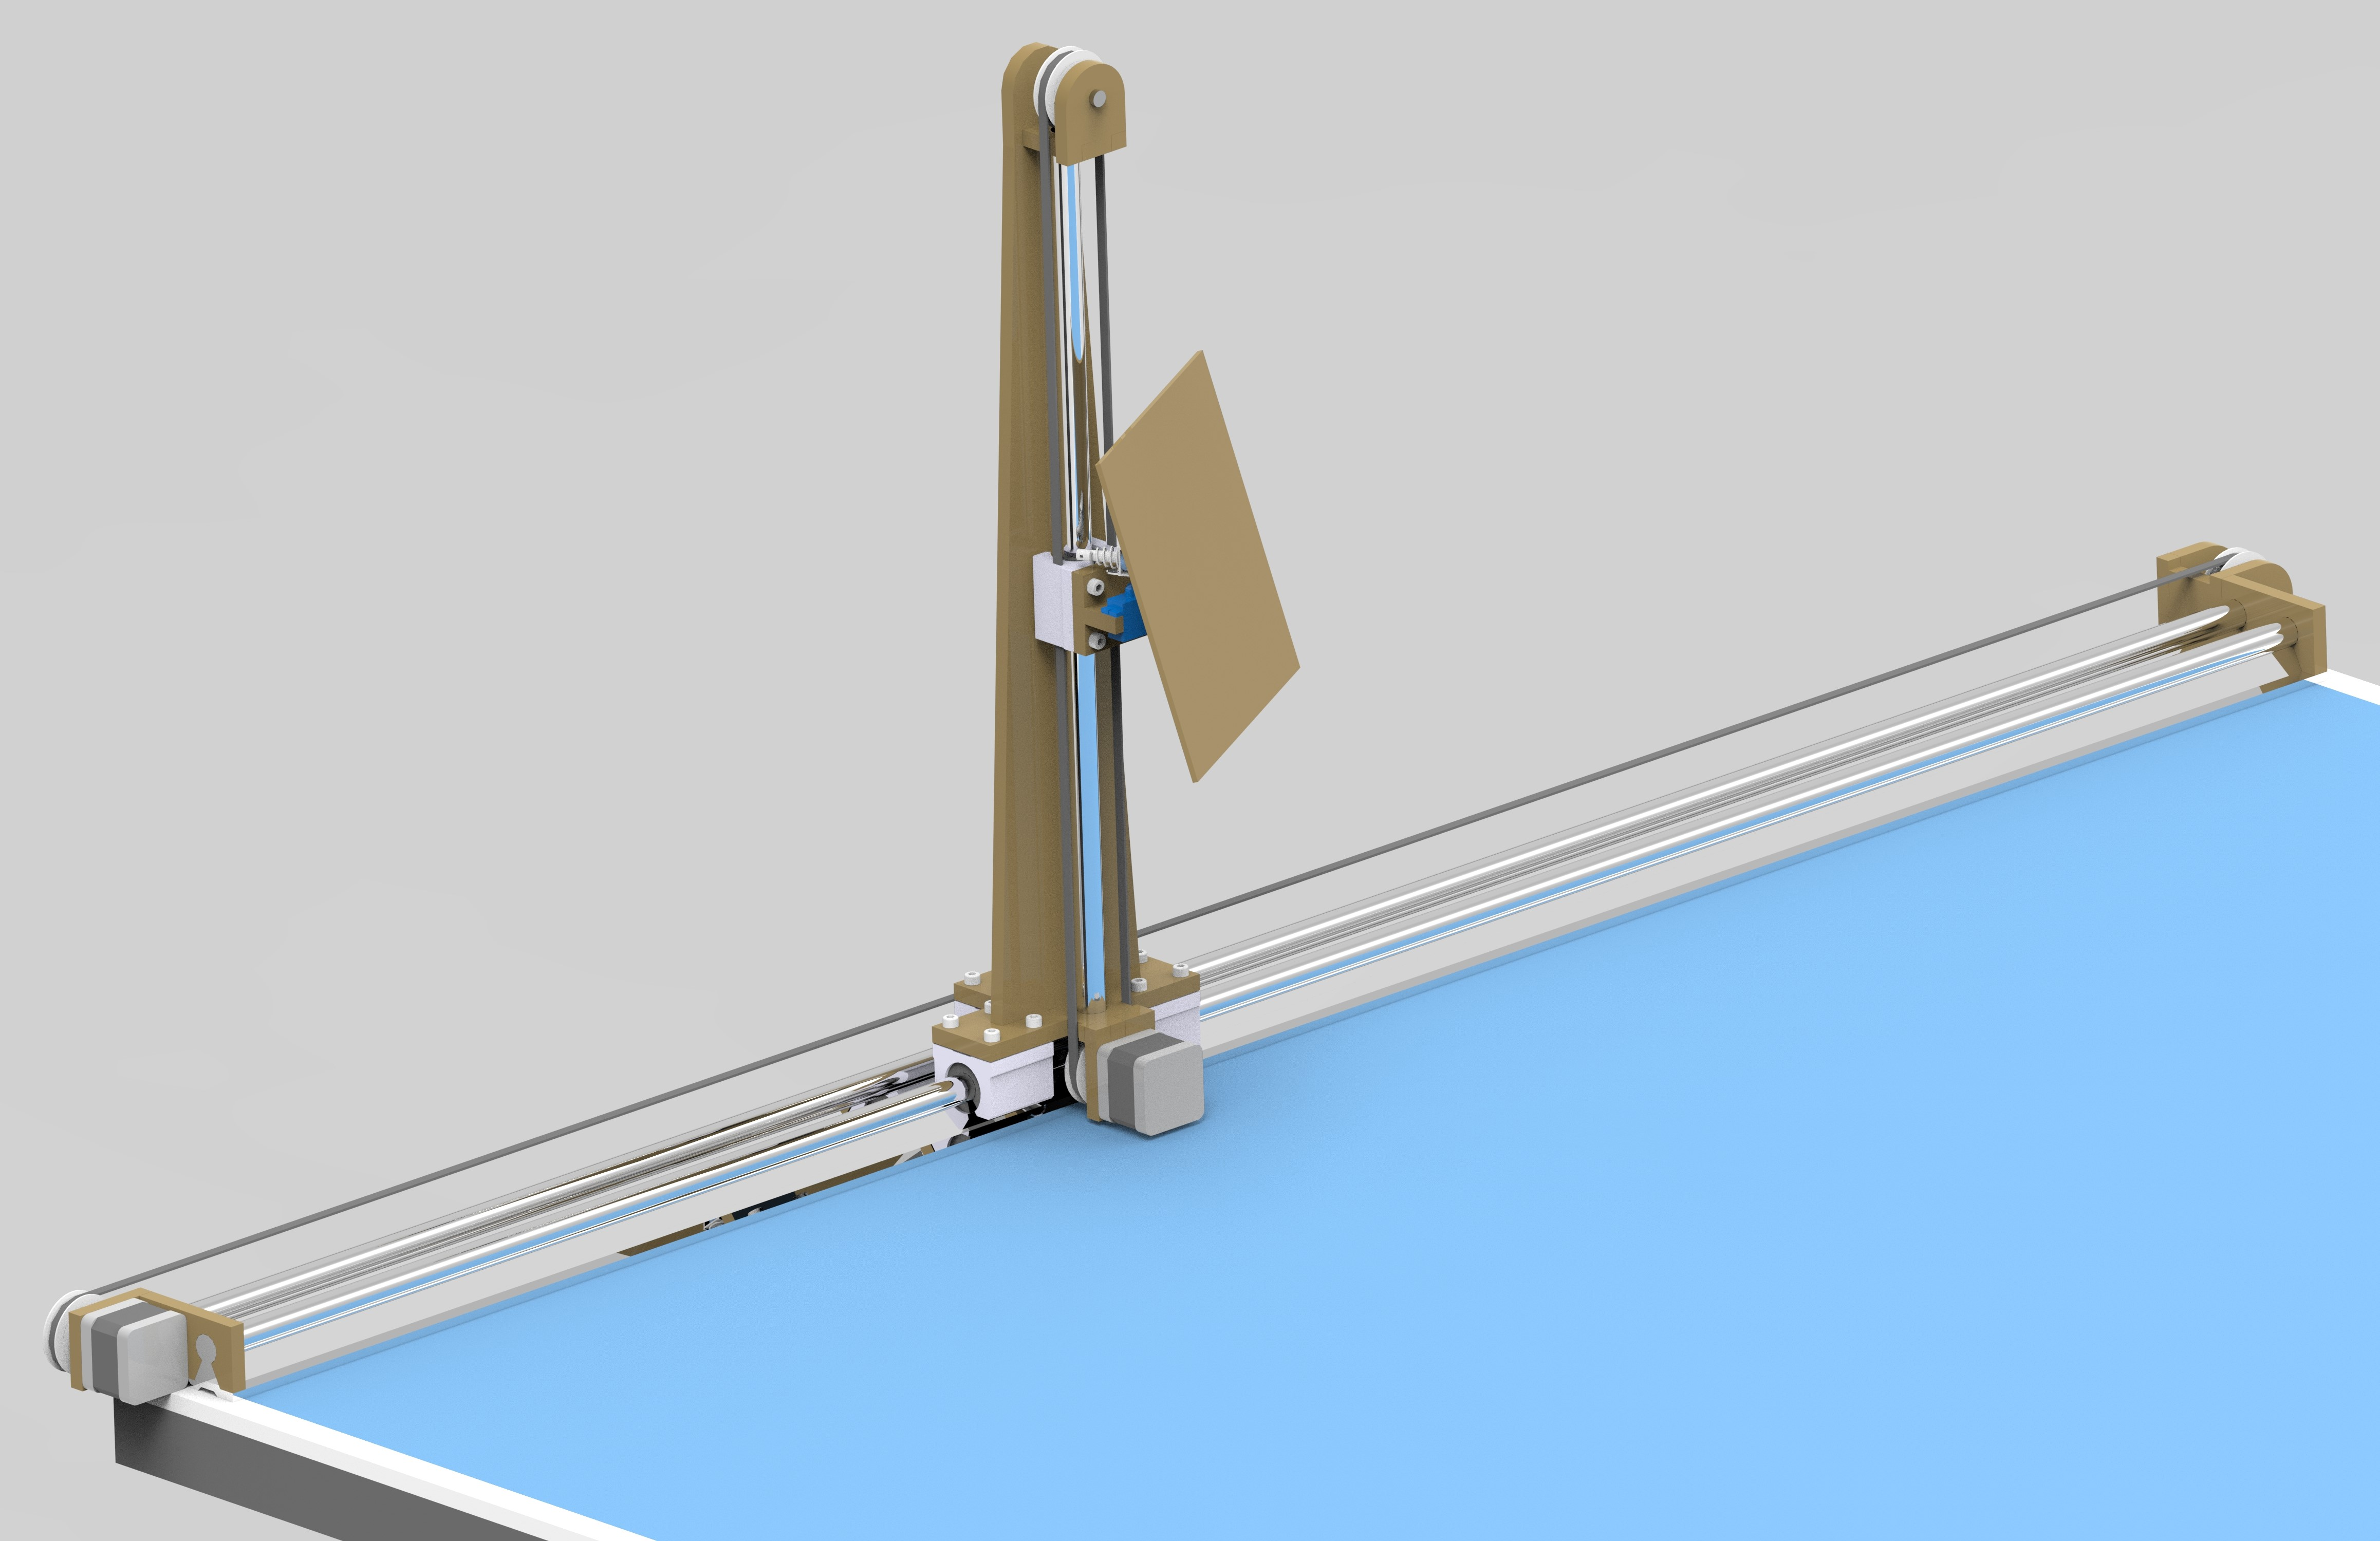
\includegraphics[height=5cm]{./images/frontrender.jpg}
	\caption{A render of the mechanical design from the front.}
\end{figure}
\begin{figure}[h] 
	\centering 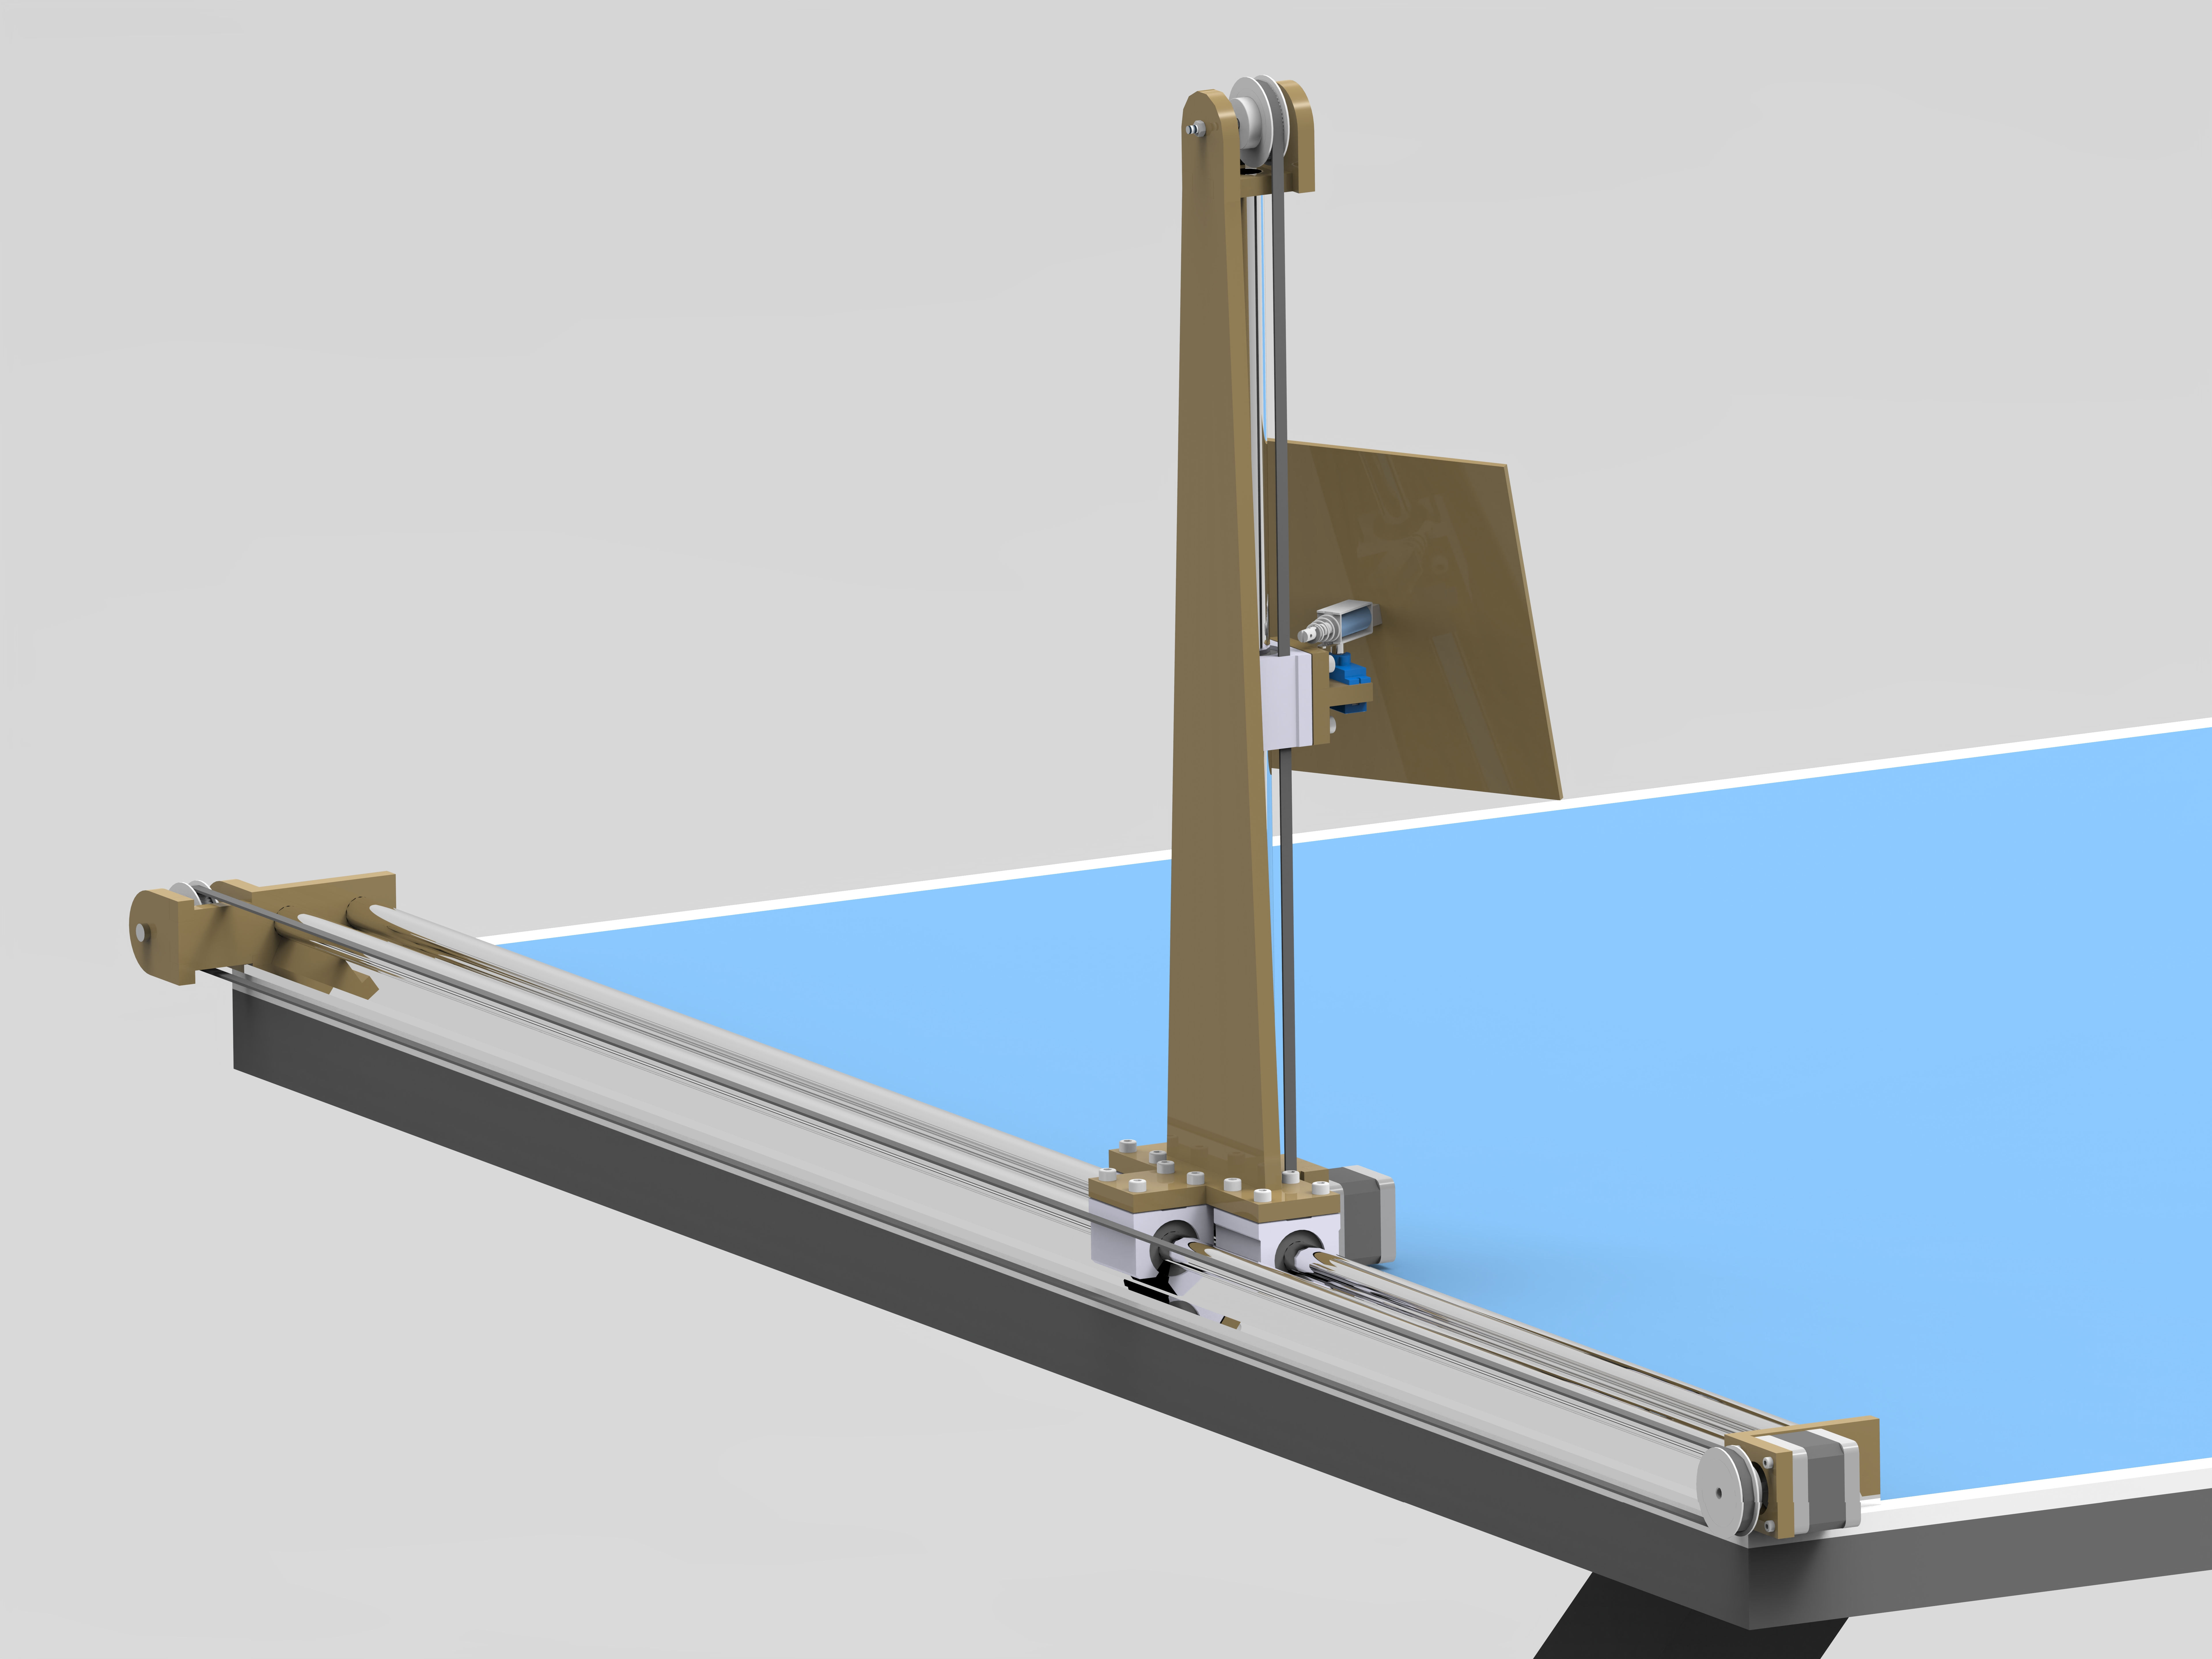
\includegraphics[height=5cm]{./images/backrender.jpg}
	\caption{A render of the mechanical design from the back.}
\end{figure}



\section{Block Diagram}
Below is a block diagram showing the general control flow of the entire system and all its components.

\begin{figure}[h]
	\centering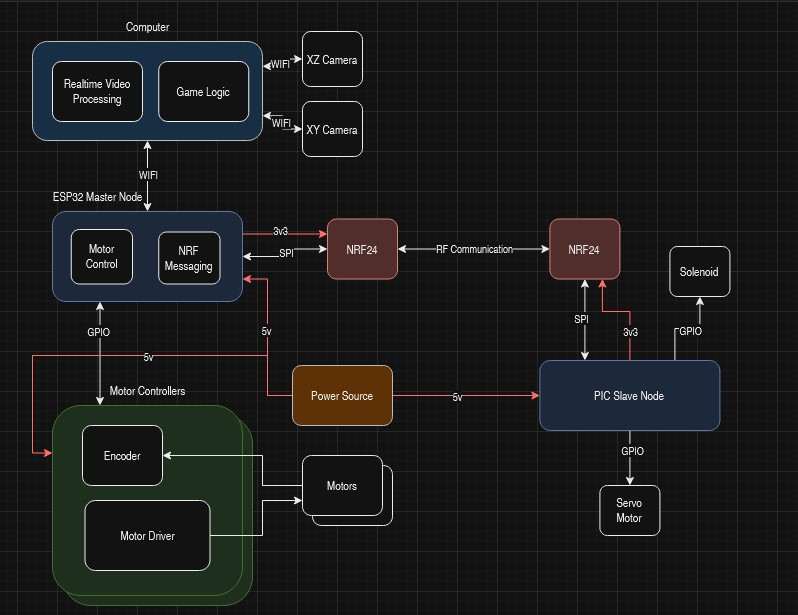
\includegraphics[height=6cm]{./images/blockdiagram}
	\caption{System Design Block Diagram}
\end{figure}

\section{Electronic Components and Controllers}
The system mainly relies on 2 mobile phones which are used for collecting the position information of the ping pong ball with 3 degrees of freedom. The mobile phones are configured with an app to act as IP cameras, which are then accessed over Wi-Fi on the control device, which is a laptop running our software.

The ESP32 microcontroller is connected to 3 stepper motor driver modules (DRV8825), which are in turn connected to 3 R.T.A. bipolar stepper motors which control the gantry. The ESP32 acts as a master to a PIC18F, though a connected radio frequency communication module (NRF24), which is used to transmit data to another NRF24 module, connected to the PIC18F slave microcontroller. This data consists of information on when to "fire" the racket to hit the ball, by activating the optocoupled 12v solenoid, and information on what angle the racket should be at, by controlling the 5v servo motor controlling the racket.

\begin{figure}[h]
	\centering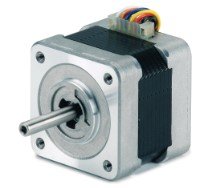
\includegraphics[height=3cm]{./images/steppermotor}
	\caption{Stepper Motor Used}
\end{figure}

\section{Software Design}
The main software which controls the system is ran on a separate computer, due to the speed constraints of small microcontrollers. The code connects to the IP camera phones, reads the streamed video data, and process it using a ball detection algorithms to determine the position of the ping pong ball in 3D space. The software sends a requested gantry position, a requested racket orientation, and when the racket should "fire" over Wi-Fi to the ESP32 microcontroller, which then sends a part of this data over radio using the NRF24 to the PIC18F.

The software additionally maintains the game state through a simplified ruleset, allowing the score and current ball position to be visualized in real time. The software determines the ball's position and additionally applies a predictive model to determine where the gantry should move to.


\section{Printed Circuit Boards}

Our design additionally consists of 2 Printed Circuit Boards (PCBs), one for each used microcontroller. The first PCB designed is for the PIC18F slave microcontroller. It contains connections for the solenoid, and its control circuit which consists of an optocoupler and a Darlington NPN bipolar transistor (TIP120). It also contains connections for the servo motor and its control circuit which is a simple MOSFET transistor circuit and contains connections for the NRF24 module.

\begin{figure}[h]
	\centering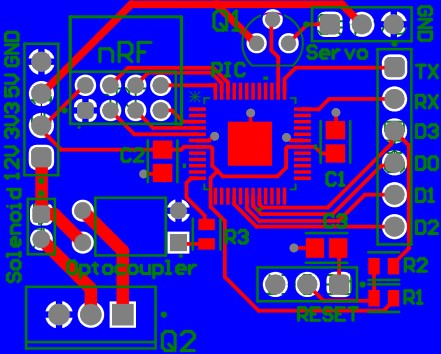
\includegraphics[height=5cm]{./images/picpcb}
	\caption{PIC18F PCB Design}
\end{figure}

The second designed PCB is for the ESP32 master controller. This PCB consists of headers for the ESP32 controller itself, and headers for each of the DRV8825 modules. It has a switch for on board adjustment of the drivers' control pins. It also contains connections for the NRF24 module.

\begin{figure}[h]
	\centering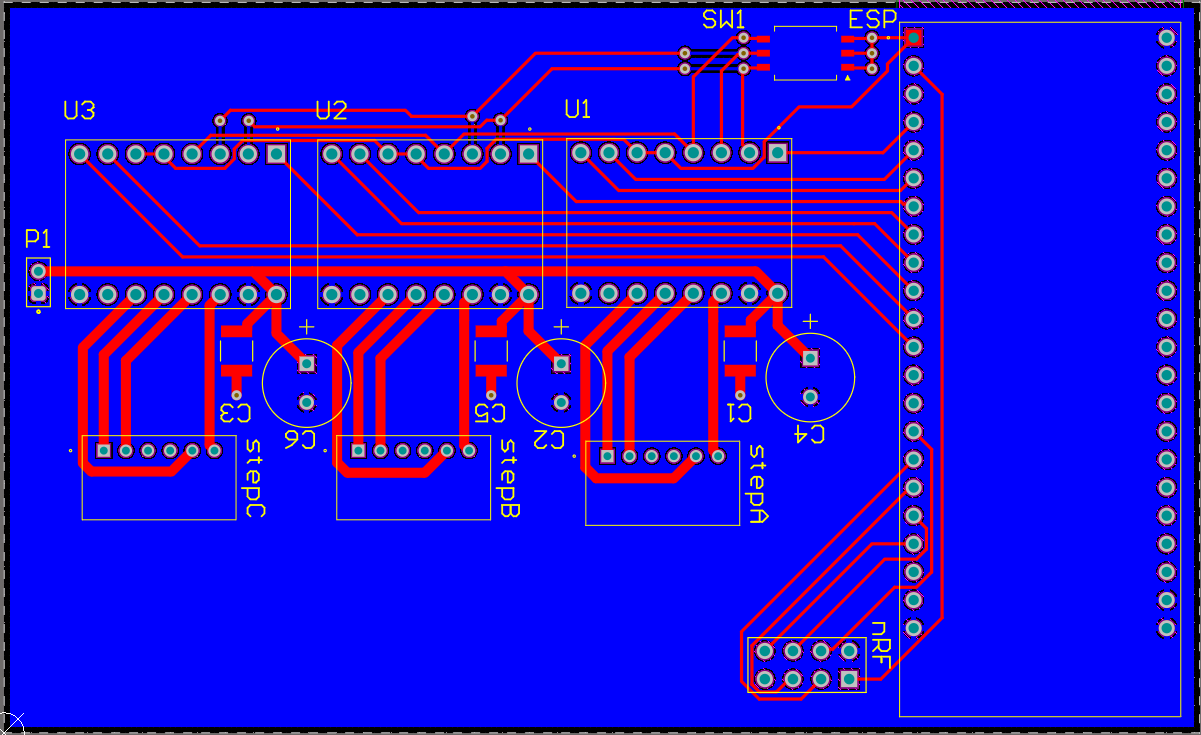
\includegraphics[height=5cm]{./images/esppcb}
	\caption{ESP32 PCB Design}
\end{figure}

\section{Bill of Materials}

\begin{center}
\begin{tabular}{|l|c|c|c|}
 \hline
Item & Amount & Price (\texteuro) \\
 \hline\hline
 MDF (60x30) & 1 & 4 \\ 
 \hline
 5meter 6mm Timing Belt & 1 & 6.62\\
 \hline
 GT2 60-tooth gear & 4 & 3.19\\
 \hline
 0.5meter M16 Aluminium pipe & 1 & 5.9\\
 \hline
 1.5meter SBR16 Linear rail & 2 & 20.46\\
 \hline
 D5 M4 50mm Shoulder bolt & 2 & 2.94\\
 \hline
 Servo Motor & 1 & 3.5 \\
 \hline
 Solenoid & 1 & 6.9 \\ 
 \hline
 ESP32 & 1 & 6.9 \\
 \hline
 PIC18F & 1 & 2.4 \\
 \hline
 NRF24 & 2 & 6.68 \\
 \hline
 Stepper Motor & 3 & - \\
 \hline
 Stepper Driver DRV8825 & 3 & 13.5 \\
 \hline
 Optocoupler & 1 & - \\
 \hline
 Transistors & - & - \\
 \hline
 Resistors & - & - \\
 \hline
 Capacitors & - & - \\
 \hline
\end{tabular}
\end{center}
	\chapter{Implementation}
In this section we will discuss the implementation of our previously discussed design. More specifically, the electronic hardware and software systems.

\section{Hardware implementation}
The hardware systems are implemented using two printed circuit boards (PCBs), one for each microcontroller. These handle the communication between the microcontrollers and the execution of actions, requested by the control device laptop.

\subsection{Printed Circuit Boards}

The first PCB is for the PIC18F slave microcontroller. The PIC18F resides in the middle and is the central unit of this board. The PCB contains a connection for the solenoid, to control when it need to turn on and off. It also contains connections for the servo motor and its control circuit which is a simple MOSFET transistor circuit. The board has connections for the NRF24 module, to make radio communication with the ESP32 possible. This PCB design can be seen in Figure~\ref{fig:pic-pcb}.

\begin{figure}[h]
	\centering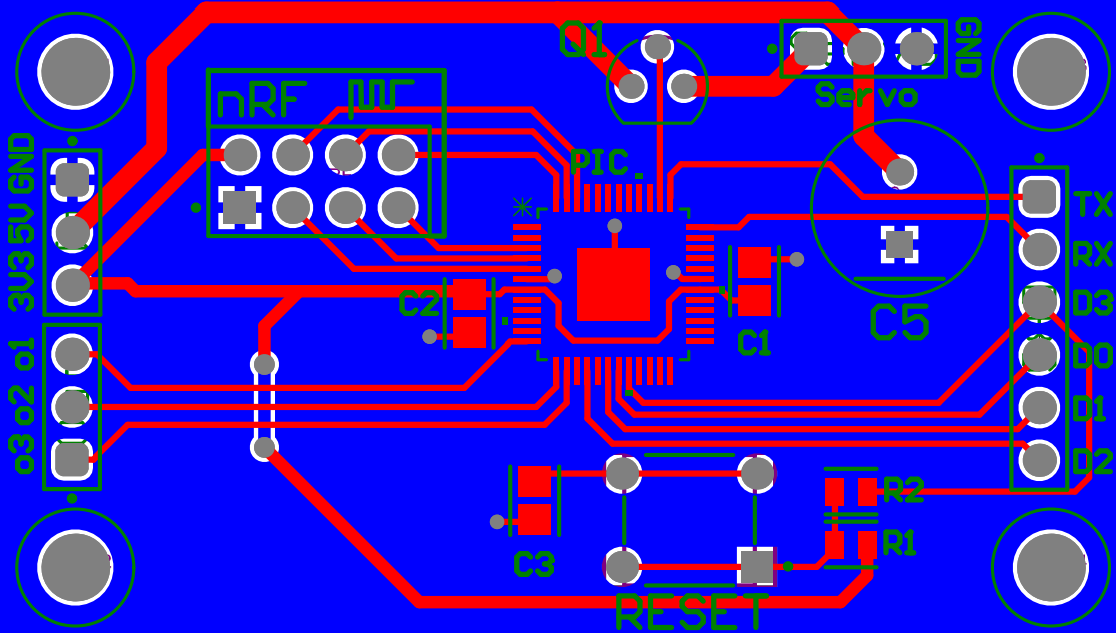
\includegraphics[height=5cm]{./images/PIC18F_pcb}
	\caption{PIC18F PCB Design}
	\label{fig:pic-pcb}
\end{figure}

The second PCB is for the ESP32 master controller. This PCB consists of pin headers for the ESP32 controller itself, and pin headers for each of the DRV8825 modules, which control the stepper motors. It has switches for on board adjustment of the drivers' control pins. It also contains connections for the NRF24 module, like the PIC18F. This PCB design can be seen in Figure~\ref{fig:esp-pcb}. 

\begin{figure}[h]
	\centering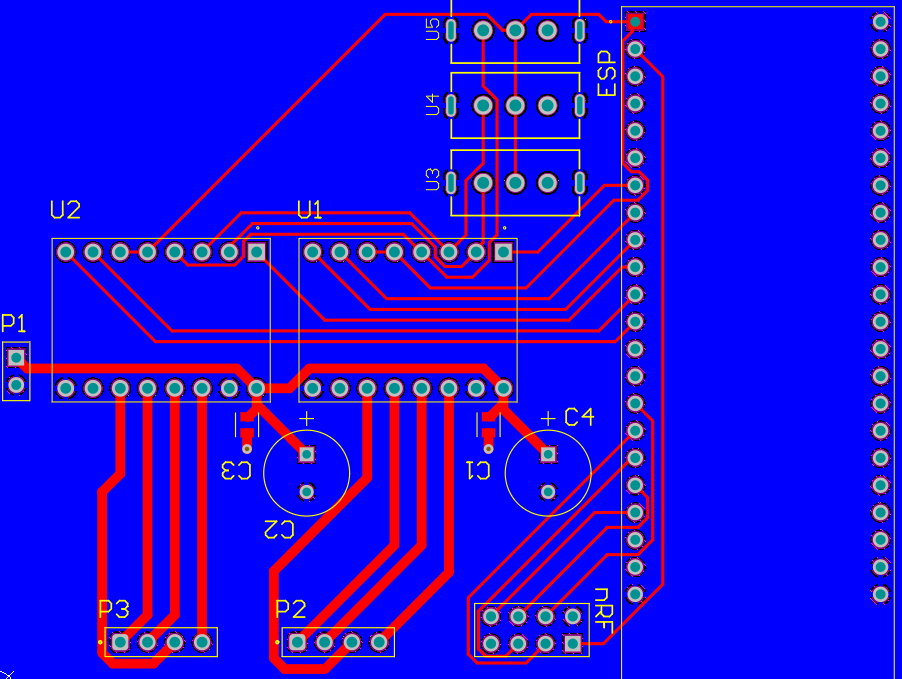
\includegraphics[height=5cm]{./images/ESP32_pcb}
	\caption{ESP32 PCB Design}
	\label{fig:esp-pcb}
\end{figure}


\section{Software implementation}

The embedded software system is developed for an ESP32-based real-time application involving motion control and wireless communication. The design follows a modular, task-based architecture utilizing the FreeRTOS operating system, allowing concurrent execution of multiple subsystems and ensuring responsiveness to real-time events.

\subsection{Architectural Overview}
The system architecture is composed of three primary subsystems: a communication subsystem, a motion control subsystem, and a simulation/testing subsystem. These subsystems interact through well-defined interfaces and communicate via FreeRTOS message queues, allowing asynchronous data exchange and decoupling between components.

\subsection{Communication Subsystem}
The communication subsystem is responsible for receiving external control commands via UDP over Wi-Fi and transmitting actuator signals through an NRF24 radio interface. The UDP client manages socket creation, data reception, and error handling, converting received commands into structured messages. These messages are placed into dedicated queues for consumption by the motion and actuator controllers. The NRF24-based radio communication provides an additional, low-latency communication channel for controlling remote actuators, contributing to the system's flexibility and scalability.

\subsection{Motion Control Subsystem}
The motion control subsystem handles the operation of two stepper motors along orthogonal axes. Motor control is implemented using hardware timers configured to trigger interrupts at precise intervals. Within the interrupt service routines, step signals are toggled, positions are updated, and step frequencies are adjusted according to desired momentum and target positions. The use of easing functions ensures smooth acceleration and deceleration, minimizing mechanical stress and enabling precise control. Position and speed adjustments are driven by messages received from the communication subsystem, allowing dynamic and responsive actuation.

\subsection{Simulation and Testing Subsystem}
To facilitate development and validation in the absence of hardware, the system incorporates a simulation and testing subsystem. Mock tasks generate synthetic messages simulating both UDP communication and actuator commands. This feature enables rigorous testing of system behavior, ensuring robustness and correctness prior to hardware deployment.

\subsection{Inter-task Communication and Decoupling}
The system employs three dedicated message queues for horizontal stepper control, vertical stepper control, and racket actuator commands. These queues enable asynchronous, thread-safe communication between tasks. The use of structured message formats for stepper and actuator commands maintains consistency and simplifies message handling logic, supporting scalability and modular expansion.

\subsection{Modularity and Configurability}
The firmware includes compile-time configuration flags to enable or disable subsystems such as UDP communication, radio communication, stepper control, and mock simulation tasks. This configurability allows the firmware to be adapted for various development and deployment scenarios, including partial module testing, hardware-in-the-loop simulations, or full production operation.

\subsection{Design Rationale}
The overall system design reflects a deliberate emphasis on separation of concerns, real-time responsiveness, scalability, and testability. The modular task-based architecture and asynchronous queue-based messaging enable the system to maintain predictable real-time behavior while remaining adaptable to future expansions or modifications. The inclusion of simulation capabilities addresses the need for verification and debugging in complex embedded systems where hardware access may be limited during certain development phases.

\subsection{Conclusion}
The software architecture presented here demonstrates an effective approach for real-time motion control and communication in an embedded environment. Through its modular design, task-based concurrency, and flexible configuration, the system achieves a balance between robustness, maintainability, and adaptability, making it well-suited for both research and applied deployment in embedded control scenarios.
	\chapter{Evaluation and validation}
This section presents a series of tests that evaluate the performance and reliability of the system. Each aspect of the system is tested to its limits in order to obtain a reliable operating range.
\section{Testing the speed limits}
To determine the maximum and minimum speed at which the prototype can move, through code, the speed of the stepper motor is gradually increased and decreased in both vertical and horizontal direction. 
We aim to identify the threshold where the performance degrades due to mechanical constraints. 
Then, through these values we can establish an optimal operating range for real-time play. 
The recorded maximum speed was around 3000 steps/second horizontally, and 400 steps/second vertically, whereas the minimum speed was 400 and 100 respectively, providing us a range for optimal robot performance.

\section{Evaluate tracking coverage}
In this stage, we are evaluating the tracking coverage of the robot's vision system by analyzing how effectively it can detect and follow the ball during a game. 
To do so, we use a pre-recorded video of the gameplay and measure the percentage of time the ball is detected versus the time it isn't. 
This will help us understand the gaps in the visual coverage, such as potential blind spots, and limitations of our tracking algorithm. 
The analysis revealed the ball was successfully tracked for 70\% of the time within the recorded data.

\section{Measure movement range}
In this part we are measuring the movement range of the robot to determine how much area is covered by the robot horizontally and vertically where the ball can be returned effectively. 
The robot is set up at the border of the ping pong table, taking into account our robot can't cover balls not reaching the end of the table. 
By observing the robot's ability to return balls from different locations on the table, the effective coverage zone and any unreachable areas can be defined. 
The testing showed the robot covered 150cm horizontally and 40cm vertically, giving us a clear idea of the physical reach.

\section{Measure Control Latency}
For this final test, we measured the response time it takes to move the robot, specifically the delay between,  pressing the button to the robot beginning to move. 
To conduct the test, we set up the robot and recorded a video capturing both a person pressing the button and the robot initial movement. 
By analyzing the video frame-by-frame we establish the time difference between input and action. 
This test will help us evaluate the system's latency, an important aspect for the real-time responsiveness of the machine. 
The measured response time was around 100ms, offering a valuable insight of the performance of our control system.

	\chapter{Discussion}
Within this project, we were able to implement the core systems needed for a ping-pong adversarial robot. The system presented shows a solid basis for building a general purpose gantry system, a robust networking architecture, a modular software suite for modeling and controlling a gantry, and a complex functional computer vision system for ball tracking and localization. To this end, we believe the system achieves its originally scoped goals of developing a framework for adversarial ping-pong automation. The developed system can move both autonomously and with a user defined manual control flow, and it is able to track game state actively with high accuracy.

 However, there were some core issues faced that prevent the system from functioning in real time as an end-to-end ping-pong system. These limitations prevent the system from being used end-to-end as is, but are mechanical/hardware issues, and were not part of the scope or intention of our experiments. Due to the nature of these issues and the ease of resolving them at a production scale, efforts were focused primarily on other sections.

\section{Latency and Speed Limitations}
Due to budgeting concerns, the system was limited to the simple stepper motors and drivers used. These motors, while somewhat powerful, are not sufficient to move the designed gantry at a speed that supports real time ping-pong. Due to this, a better solution would be to use stronger motors, ideally, non-stepper motors that allow for faster movement and higher torque. To deal with these changes, a more complex closed loop controller would have to be implemented, to support the new motors.
Furthermore, the system employed IP cameras over a Wi-Fi network, which introduce multiple layers of latency and quality issues. Due to the innate networking delays present, the system cannot transmit the image data at a rate which is sufficient for the requirements, which can be a bottleneck for the autonomous modes. Switching these cameras out for dedicated cameras would significantly improve the performance at a cheap cost.
Additionally, the system employed the use of radio frequency communication NRF modules, which added another level of latency. These modules can be replaced by direct wired UART communication between microcontrollers, further increasing the reactivity of the system.
Finally, the system applies its image processing on a computer running a python OpenCV powered processing algorithm. This system can be implemented directly on a microcontroller, or in a more optimized desktop environment if necessary, to improve the speed of processing further. Additionally, the data from computer to the gantry was sent via Wi-Fi, this could be replaced by serial communication for lower latency.

\section{Hardware Limitations}
Since the system was a prototype built with heavy time constraints, heavily adjusting the mechanical system was not an option. Because of this, the prototype is fully functional, but can be improved in many ways. The system has many points with heavy friction, which increases the load the motors have to deal with. Furthermore, the gantry faces some stability issues, due to the cheap materials and lack of supports.
Another issue faced was the low force applied by the solenoid racket system. This is due to the solenoid being ineffective at providing the required force. The intended alternative for this solenoid was a motor-driven spring-loaded linear actuator, however that was scrapped for the convenience of the solenoid. For this proof of concept system, the solenoid performed as expected.
	\chapter{Conclusion}
To conclude, in this paper we explore the process of implementing a robust and reconfigurable adversarial ping-pong robot. We show that it is possible to develop a cheap ping pong robot within some constraints, and provide solutions to any ongoing issues. We provide the basis for implementing a general purpose gantry with a reconfigurable and powerful software suite, and show the possibilities of real time ping-pong within computer vision.

	%%% Bibliography: references. included from bibliography.bib
	%%% Only referenced items are displayed in the final document
	%\nocite{*}			% if you also want to display the unreferenced items in your bibliografy uncomment this
	\bibliographystyle{ieeetr}
	\bibliography{bibliography}

	%%% appendices
    \appendix
    \appendixpage
	% when you are using the twocolumn layout for your thesis appendixes may/can be in a 'singlecolumnsection'
\begin{singlecolumnsection}
\chapter{Some extra info}

Delete the appendix if not needed.

\end{singlecolumnsection}

	%%% Apendix from other pdf
%	\chapter{Poster}
%	\includepdf{poster.pdf}

	\backcover
\end{document}
